\documentclass[
  a4paper,
  emulatestandardclasses,
  abstract,
  parskip,
  appendixprefix,
  listof=totoc,
  bibliography=totoc
]{scrreprt}

\usepackage[ngerman,english]{babel}

\usepackage{bm}
\usepackage{xcolor}
\usepackage{a4wide}
\usepackage{authblk}
\usepackage{physics}
\usepackage{amsthm}
\usepackage{amsmath}
\usepackage{amssymb}
\usepackage{csquotes}
\usepackage{caption}
\usepackage{biblatex}
\usepackage{enumerate}
\usepackage{graphicx}
\usepackage{hyperref}
\usepackage{cleveref}
\usepackage[
  binary-units
]{siunitx}
\usepackage[
  acronym,
  nonumberlist,
  toc,
  nohypertypes={acronym}
]{glossaries}
\usepackage{unicode-math}

\addbibresource{literature.bib}

\makeglossaries
\newacronym{rf}{RF}{radio frequency}
\newacronym{smf}{SMF}{single-mode optical fiber}
\newacronym{aom}{AOM}{acousto-optic modulator}
\newacronym{aod}{AOD}{acousto-optic deflector}
\newacronym{dds}{DDS}{direct-digital synthesizer}
\newacronym{ccd}{CCD}{charge-coupled device}
\newacronym{ic}{IC}{integrated circuit}
\newacronym{pll}{PLL}{phase-locked-loop}
\newacronym{ad9910}{AD9910}{direct-digital synthesizer from Analog Devices}
\newacronym{asf}{ASF}{amplitude scale factor}
\newacronym{ftw}{FTW}{frequency tuning word}
\glsaddall

\subject{Many Body Quantum Optics}
\title{High-precision time-averaged optical potentials for ultracold atoms}
\subtitle{Bachelor thesis by}
\author[1]{Bodo Kaiser}
\affil[1]{Ludwig-Maximilians-Universität München}
\affil[ ]{\textit{bodo.kaiser@physik.uni-muenchen.de}}
\publishers{originated under the supervision of Prof. Dr. Immanuel Block,\\
  Dr. Monika Aidelsburger and Christian Schweitzer.}

\begin{document}

\makeatletter
\begin{titlepage}
  \begin{center}
    \usekomafont{subject}
    \@subject

    \vspace{.8em}
    \usekomafont{title}\huge
    \@title

    \vspace{.5em}
    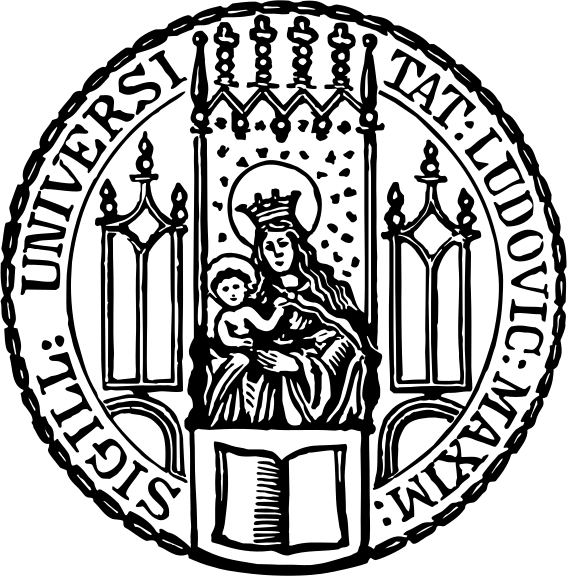
\includegraphics[width=.5\pagewidth]{build/emblem.pdf}

    \usekomafont{subtitle}
    \@subtitle

    \vspace{.8em}
    \usekomafont{author}
    \@author

    \usekomafont{date}
    \@date

    \vspace{.8em}
    \usekomafont{publishers}
    \@publishers
  \end{center}
\end{titlepage}
\makeatother

\makeatletter
\begin{titlepage}
  \begin{otherlanguage}{ngerman}
    \begin{center}
      \usekomafont{subject}
      Mehrteilchen Quantenoptik

      \vspace{.8em}
      \usekomafont{title}\huge
      Hochpräzise zeitgemittelte optische Potentiale für ultrakalte Atome

      \vspace{.5em}
      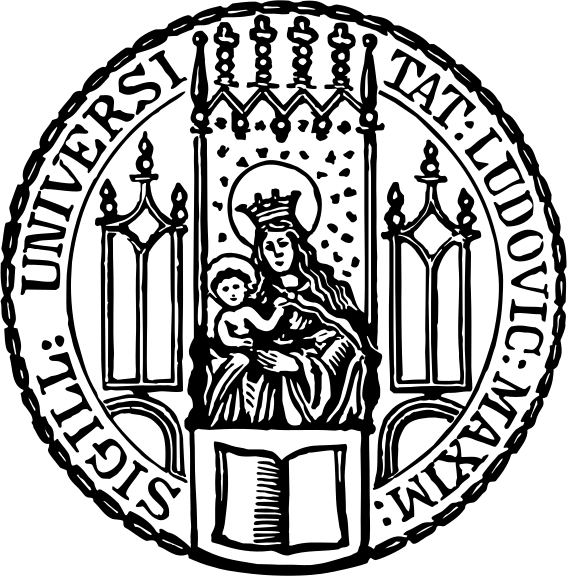
\includegraphics[width=.5\pagewidth]{build/emblem.pdf}

      \usekomafont{subtitle}
      Bachelorarbeit von

      \vspace{.8em}
      \usekomafont{author}
      \@author

      \usekomafont{date}
      \@date

      \vspace{.8em}
      \usekomafont{publishers}
      entstanden unter der Betreuung von Prof. Dr. Immanuel Block,\\
      Dr. Monika Aidelsburger und Christian Schweitzer.
    \end{center}
  \end{otherlanguage}
\end{titlepage}
\makeatother

\addchap{Acknowledgement}

The success and final outcome of the present work required a lot of guidance
and assistance from many people, without them it would not have been possible
for me to deliver this piece of work and look back on to the exciting,
enriching and diverse experience made in the last weeks, and I would not
forget to thank them.

At most I want to thank my parents for their support, that I have been
privileged to benefit from all the years. Though my life involved many
unexpected turnarounds, I never felt left alone and could rely on your
diverse experience.

Further I want to thank Prof. Bloch and Dr. Aidelsburger for creating and
sustaining a fertile scientific environment that allows inspiring discussions
at almost any time as well as seamless implementation of new ideas. Equally I
want to express my gratitude to all personal involved in the formation process
of my thesis. Especially I want to name Christian Schweizer, Hendrik v. Raven
and Till Klostermann who were available for any questions but also open to
fun from time to time. Finally I want to thank Bodo Hecker for any electronic
specific advise.

I also owe my deep gratitude to XY, who have been so friendly to check this
thesis against all sort of language abuses and offer a wide range of
suggestions to improve the expressiveness.

\addchap{Declearation of Authorship}

\addsec{Statutory Declearation}

I hereby declare that this thesis has been composed solely by myself except
where indicated otherwise by reference or acknowledgment.

The work presented has not been submitted, in whole or in part, in any
previous application for a degree.

\vspace{1em}
\textbf{Munich, \today}

\begin{abstract}
Lorem ipsum dolor sit amet, consectetur adipisici elit,
sed eiusmod tempor incidunt ut labore et dolore magna aliqua. Ut enim ad
minim veniam, quis nostrud exercitation ullamco laboris nisi ut aliquid ex ea
commodi consequat. Quis aute iure reprehenderit in voluptate velit esse
cillum dolore eu fugiat nulla pariatur. Excepteur sint obcaecat cupiditat
non proident, sunt in culpa qui officia deserunt mollit anim id est laborum.
\end{abstract}


\tableofcontents

\chapter{Introduction}

Many quantum systems studied in condensed matter physics are experimentally
challenging to access as any interactions can destroy the carefully prepared
quantum states. As way forward, experiments with ultracold atoms in
optical lattices give us a highly contorllable environment, giving us the
opportunity to simulate and explore quantum effects and expand our current
understanding of quantum mechanics and statistical physics \cite{Gross2017}.

The central idea behind these types of experiments is to cool down neutral
atoms to micro Kelvin and below, and load them into an optical lattice. At
these temperatures atoms demonstrate quantum behaviour. The optical lattices
act as periodic potentials analogue to the periodic potential found inside
solid state crystal lattices \cite{Lewenstein2007}. Unlike to i.e. real solids
where we have limited prospects to amend a systems properties, lasers driven
by state of the art optics and electronics give us a wide range of well
controllable parameters.

\begin{figure}[h]
  \centering
  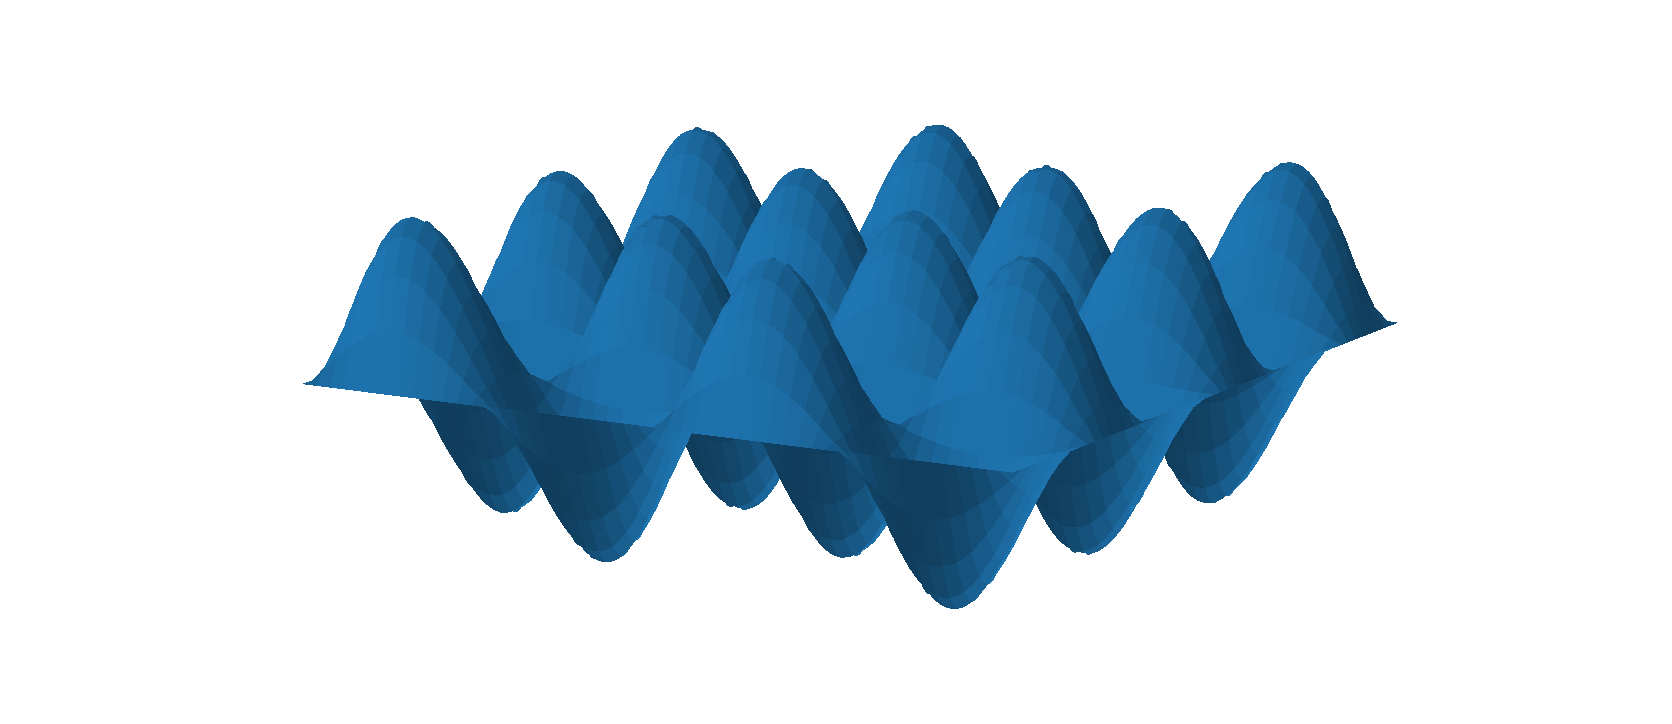
\includegraphics[width=.8\textwidth]{images/optlat/default.pdf}
  \captionsetup{width=.8\textwidth}
  \caption{Periodic potential of a 2D optical lattice. If the kinetic energy
  of the atoms is below the potential energy of the lattice, the atoms will
  locate around the potential minimas.}
  \label{fig:optlat}
\end{figure}

One of the parameters of interest is the ability to apply local potentials
to the system, that can be used to, among others, study lattice inpurities
or quantum interactions. In this work we will present and characterize one
possible implementation of such a local potential generating apparatus.

\section{Related Work}

Local manipulations of atoms inside optical lattices have been known for some
time in the embodiment of optical tweezers that allow trapping, stacking and
sorting of particles \cite{Tadmor2004}. Yet, only recently attempts to
interact with local particle clusters through high-precision time-averaged
optical potentials have been reported \cite{Roy2016}.

In the following we continue on the laid out work \cite{Hertlein2017} which
provided us with an optical setup for single-site manipulation using
\gls{aod} as well as considerations with regard to aperture limited
gaussian beam propagation.

\chapter{Experimental Setup}

The exerimental setup was largely adopted from \cite{Hertlein2017}. Amendments
made include the \gls{rf} signal source of the \gls{aod} and an additional
photodiode to measure the deflected beam intensity.

\section{Optics}

The optical setup can be dissect into two sections. The first section reduces
the power of the $\SI{532}{\nano\meter}$ laser source from $\SI{10}{\watt}$
to below $\SI{2}{\milli\watt}$ for the purpose of safe operation of an open
deflection setup, the second section. Both sections are connected through a
\gls{smf}.

\subsection{Power Reduction}

For safety reasons the power reduction setup, Figure~\ref{fig:powerbox},
is confined into a visually sealed superstructure.

\begin{figure}[h]
  \centering
  \includegraphics[width=\textwidth]{\builddir{powerbox.pdf}}
  \caption{Optical configuration of the power reduction box.}
  \label{fig:powerbox}
\end{figure}

The laser beam leaving the laser source is polarized by a $\lambda/2$ retarder
plate such that the succeeding high power beamsplitter BS can divert a large
part of the power into a beam dump.

Afterwards mirrors M1 and M2 direct the beam towards the center of a
$2:1$ telescope composed of two lenses L1, L2 with focal length
$f_1=\SI{100}{\milli\meter}$ and $f_2=\SI{50}{\milli\meter}$.

An \gls{aom} diffracts the laser collimated laser beam into multiple orders.
Mirrors M3, M4 project theses orders onto a pinhole which is adjusted to
absorb all orders except for the first order. The intensity of the first order
is subject to the amplitude signal apllied to the \gls{aom}.

Finally a tunable $\lambda/2$ retarder plate can be used to couple the beam
polarization with the \gls{smf}.

\subsection{Beam Deflection and Detection}

From the \gls{smf} the setup for beam deflection and detection,
Figure~\ref{fig:deflection}, now receives the downpowered beam through a
fiber coupler. Hereinafter a tunable retarder plate with beam splitter BS1
can be used to adjust the beam intensity without having to access the power
box. A second polarizer with cube BS2 is used to branch off part of the beam
to a photodiode PD1. We will describe later how said photodiode is used for
intensity control.

\begin{figure}[h]
  \centering
  \includegraphics[width=\textwidth]{\builddir{deflection.pdf}}
  \caption{Optical configuration of the main setup section.}
  \label{fig:deflection}
\end{figure}

Two \gls{aom} are used for vertical and horizontal beam deflection as a
function of applied frequency pairs. From hereon a $1:1$ telescope comprised
of two lenses L1, L2 with focal length $f_1=f_2=\SI{250}{\milli\meter}$
projects the laser bean on a pair of objectives that represent the atom
plane of our later experiment. The objectives are configured so that the
laser can exit unaltered.

The laser beam is reflected by a pair of mirrors M3, M4 to the part intended
for detection. Lens L3 acts as a camera lens and projects the beam to infinite
focus. Cube BS3 forks a portion of the beam away from the CCD camera on to
mirror M5 that reflects the beam towards lens L4 that focuses the beam onto
photodiode PD2.

\section{Electronics}

\subsection{Signal Source}

\subsection{Intensity Stabilizer}

\chapter{Calibration}

Alterations of the laboratory environment combined with the exchange of
components from the original setup made it advisable to recalibrate the setup.
In this chapter we want to document the steps necessary for calibration for
successive experiments.

\section{Fiber Coupling}

The visually shielded section of the setup used to reduce the output power
of the laser source is optically paired with the open section for beam
deflection via a \gls{smf} that only permits two orthogonal polarization and
a single gaussian mode. Through tuning the polarisator inside the power
reduction section we can try to match one of the orthogonal polarization
modes supported by the \gls{smf}. Polarization discrepancies induce the
polarization inside the \gls{smf} to oscillate on environmental changes like
temperature or vibration. Henceforth it is key to couple polarization modes
in order to ensure a stable operation.

The following receipt has proven to be successful to find an approximate
polarization match between the laser beam and the \gls{smf}. In addition
to the setup described in \cref{sec:powerbox} and \cref{sec:deflection}
an oscilloscope and a hot air gun are highly recommended.

\begin{enumerate}
  \item Connect the photodiode to the oscilloscope and use a coarse time
    scale of i.e. \SI{2}{\second}.
  \item Apply safety measures i.e. put on appropiete laser safety glasses and
    inform present personal of the imminent danger.
  \item Open the cover of the power reduction setup.
  \item Apply heat to the \gls{smf} through the hot air gun, alternatively
    you can try to move the fiber.
  \item The photodiode signal should start to oscillate. Tune the polarizor
    inside the power reduction subject to minimizing the oscillation.
\end{enumerate}

The oscillations occur as the polarization circulates inside the fiber and
will stop at some point. In this case yu should remove the heat or mechanical 
stress on the fiber and wait some time before you can reapply with the initial
response.

\section{Beam Alignment}

As is well known, beams that pass off-centered through spherical lenses
experience optical aberrations. Additionally we found that uncentered beams
may cause further optical defects from reflections at boundaries. Both effects
should be avoided as far as possible by adjusting positions and mirror angles.

As auxilliaries we recommend a pair of iris diaphragms that are mountable to
the lens mounts and a screen i.e. a white sheet of hard paper. With the iris
diaphragms we can easily find a center reference point visually by inspecting
the symmetry of the iris illumination at different pinhole diameters. Exact
steps are summarized in the below receipt. We refer to the optics as annotated
in \cref{fig:deflection}.

\begin{enumerate}
  \item Place screen in front of L2 and adjust screws on fiber coupler subject
    to a clean beam profile on the screen of the (1,1) diffraction order of
    the \gls{aom}s.
  \item Apply one iris to L2 and find center frequency of the \gls{aom}s.
  \item Mount irises on L3 and L4. Mount mirror pair M1, M2 to direct beam
    through both pinholes.
  \item Place auxilliary lens with mounted iris between L7 and M3 and adjust
    second objective pair L6, L7.
  \item Mount iris on L8 and place auxilliary lens with mounted iris in front
    of BS3. Align the mirror pair M3 and M4 to reflect the beam through both
    irises.
  \item Adjust the objective pair distance until you see an output similar to
    XY on the \gls{ccd} camera.
\end{enumerate}

The alignment of a mirror pair can be simplified by using the below algorithm:

\begin{enumerate}
  \item Select axis to align.
  \item Align the beam on the outside lens by tuning the inner mirror.
  \item Align the beam on the inner lens by tuning the outside mirror.
  \item Repeat steps 2 and 3 until beam is aligned on both lenses. Proceed
    with other axis.
\end{enumerate}

\section{Camera Focus}

Finally we had to reposition the camera to focus the incoming beam correctly
in order to register the beam profile as would be seen later by the atoms.
To find the precise focus position we followed the procedure described in
\cite{Hertlein2017} that consits of extracting the camera rail with its lens
and focusing it on a far distant object.

\begin{figure}[ht]
  \centering
  \includegraphics[width=\textwidth]{\builddir{focus.pdf}}
  \caption{Camera focused on far distant object. In this case a window from the
  building accross the courtyard.}
\end{figure}

\section{Beam Profile}

% Image from CCD camera with gaussian fit

\chapter{Measurements}

% computer -> dds
%          -> scope
%          -> trigger
%          <- scope

\section{Electronics}

\subsection{Signal Source}

\subsection{Signal Amplifier}

% network analyzer (frequency dependence amplification)
% chirp signal deviation from ideal

\subsection{Intensity Control}

% test of long time stability

\section{Acousto-Optics}

\subsection{1D Intensity Distribution}

% H removed, V sweep (H in V position, vice versa)
% V removed, H sweep (V in H position, vice versa)

% H constant with V sweep
% V constant with H sweep

% amplitude modulation

\subsection{2D Intensity Distribution}

% without amplitude modulation
% with amplitude modulation

\chapter{Conclusion}

\section{Summary}

\section{Future Outlook}

\section{Further Applications}


\printglossaries
\listoffigures
\listoftables
\printbibliography

\appendix
\chapter{Electronics}

\section{Trigger Hub}
\label{app:electronics:trigger_hub}

The trigger hub is driven by a \SI{3.3}{\volt} input signal and a
\SI{5}{\volt} voltage source. The input signal is amplified to drive four
\gls{ttl} inputs through use of the \gls{sn74128} \cite{SN74128} line driver.
Furthermore the hub is designed to be mounted on the \gls{bbb} which itself
provides the trigger network interface.

\begin{figure}[h]
  \centering
  \captionsetup{width=.8\textwidth}
  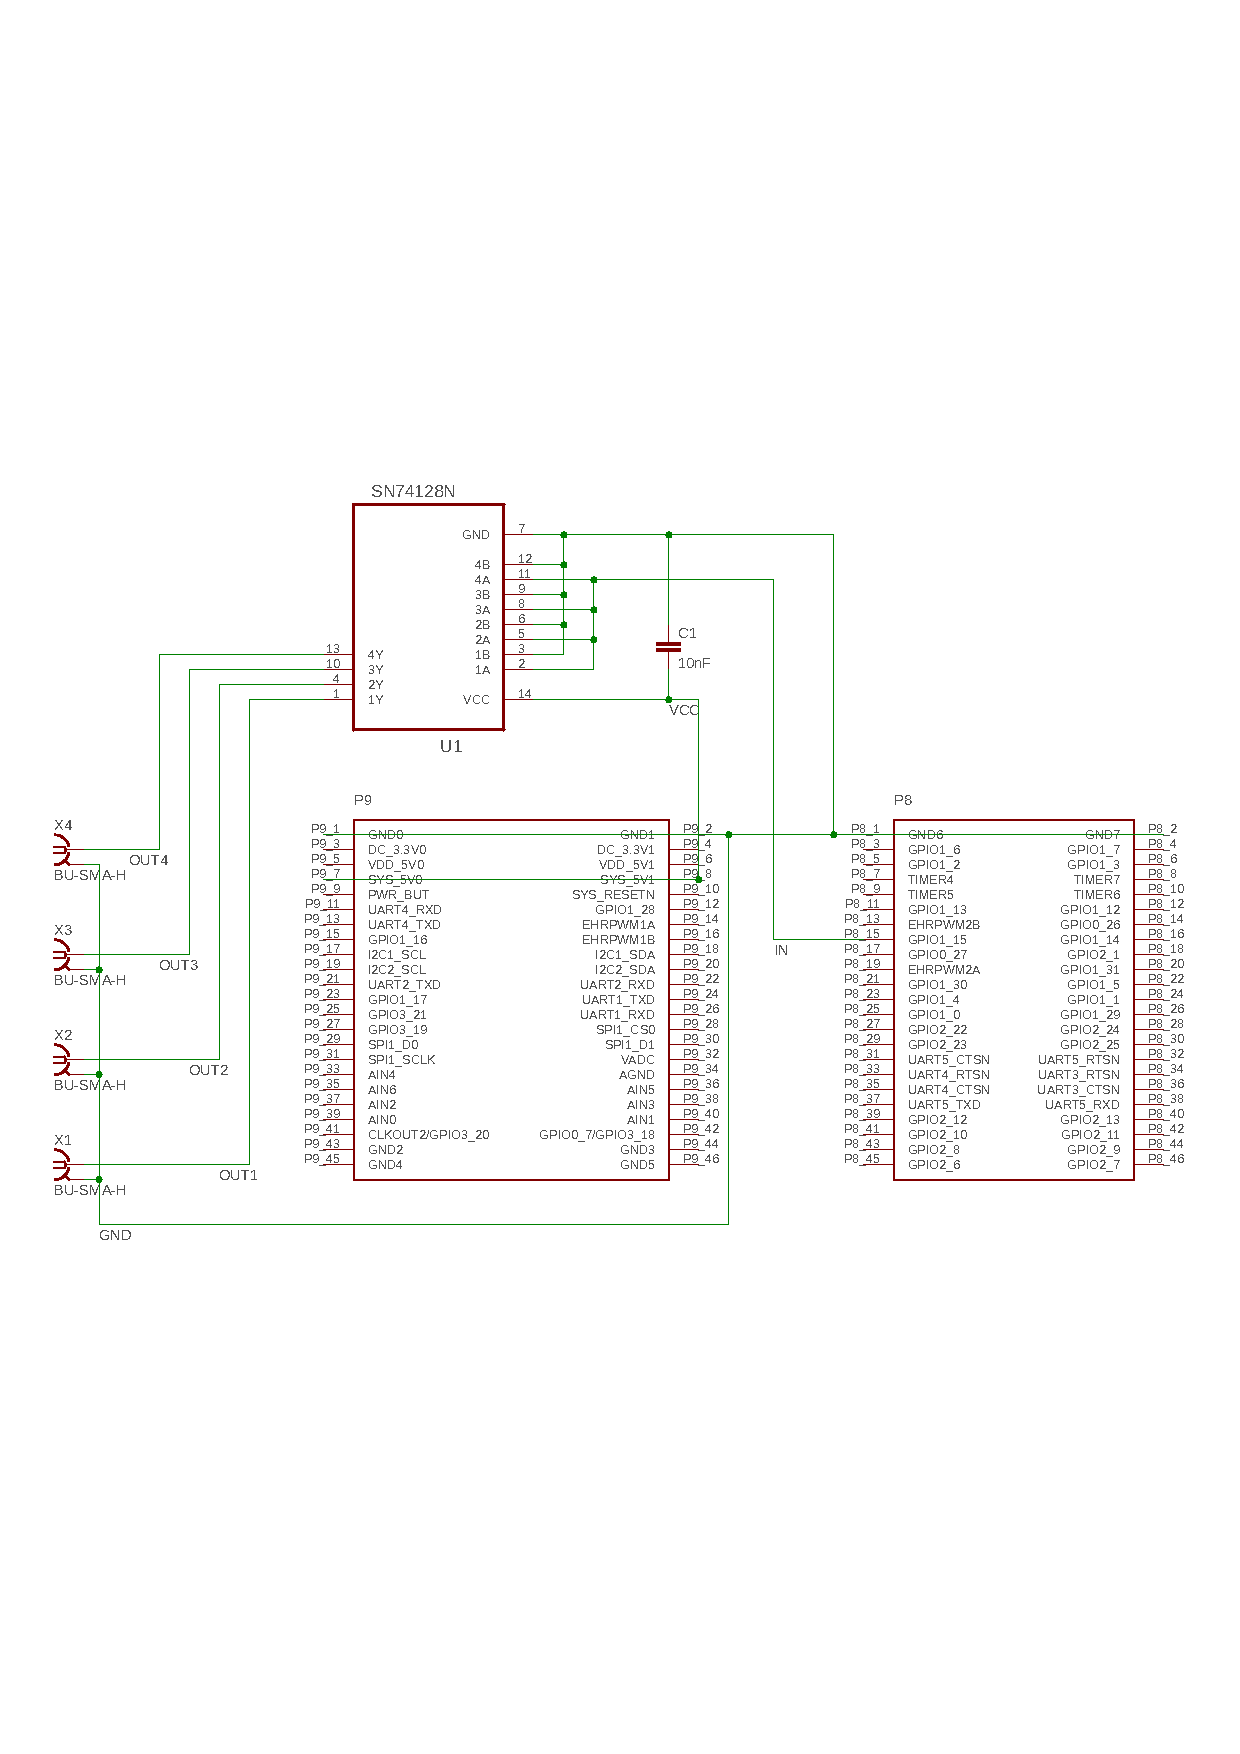
\includegraphics[width=\textwidth]{images/circuits/line-driver/schematic.pdf}
  \caption{Elecronic circuit schematics of the trigger hub. The
    \SI{3.3}{\volt} input signal is amplified by the \gls{sn74128} line
    driver and outputed to four \gls{sma} connectors.}
\end{figure}

The \gls{sn74128} exposes four independent outputs $Y$, each is driven by a
two-input ($A$ and $B$) with NOR ($\overline{A+B}=Y$) logic. As our objective
is to forward rising edge trigger signals we pulled all four $B$ to low by
connecting them with \gls{gnd}. The four $A$ where connected together with
the input signal. The input signal has to transition from $1$ to $0$ in order
to signal a rising edge trigger signal.

\begin{listing}[h]
  \inputminted[xleftmargin=.2\linewidth]{javascript}{scripts/trigger.js}
  \captionsetup{width=.6\linewidth}
  \caption{\gls{bbb} script that starts a \gls{http} server to listen for
requests on which to trigger a rising edge signal. On execution it pulls the
signal \gls{gpio} to high. The request callback then pulls the \gls{gpio} to
low for one \SI{1}{\milli\second}.}
\end{listing}

Using the \gls{bbb} makes it easy to write scripts that communicate with
other devices over the \gls{lan}. We used the bonescript library to access
the \gls{gpio} interface as it is pre-installed on the \gls{bbb}.

\begin{figure}[h]
  \centering
  \begin{minipage}{.40\textwidth}
    \centering
    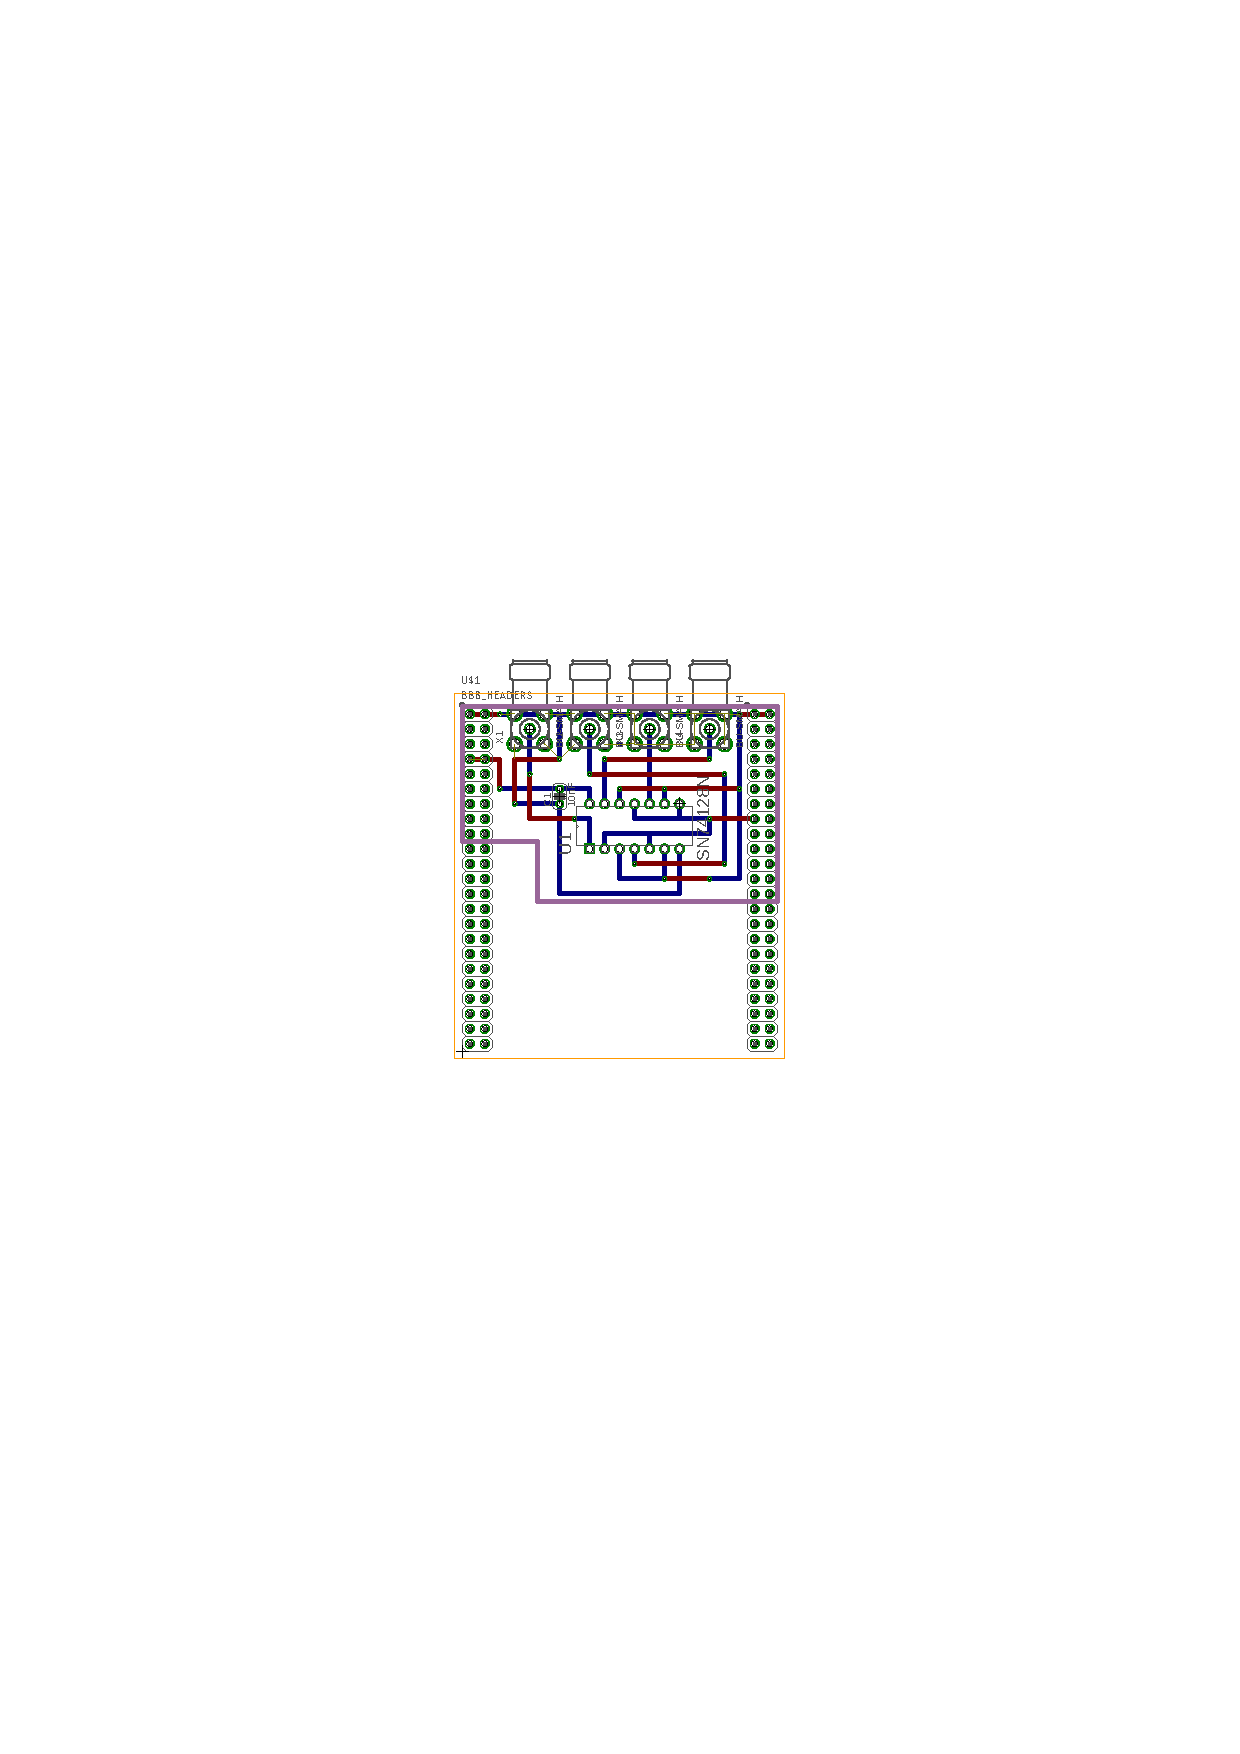
\includegraphics[width=\linewidth]{images/circuits/line-driver/layout.pdf}
    \captionsetup{width=\linewidth}
    \caption{Board layout of the trigger hub. The source amplifier is designed
to fit on top of the \gls{bbb} expansion headers.}
  \end{minipage}
  \begin{minipage}{.50\textwidth}
    \centering
    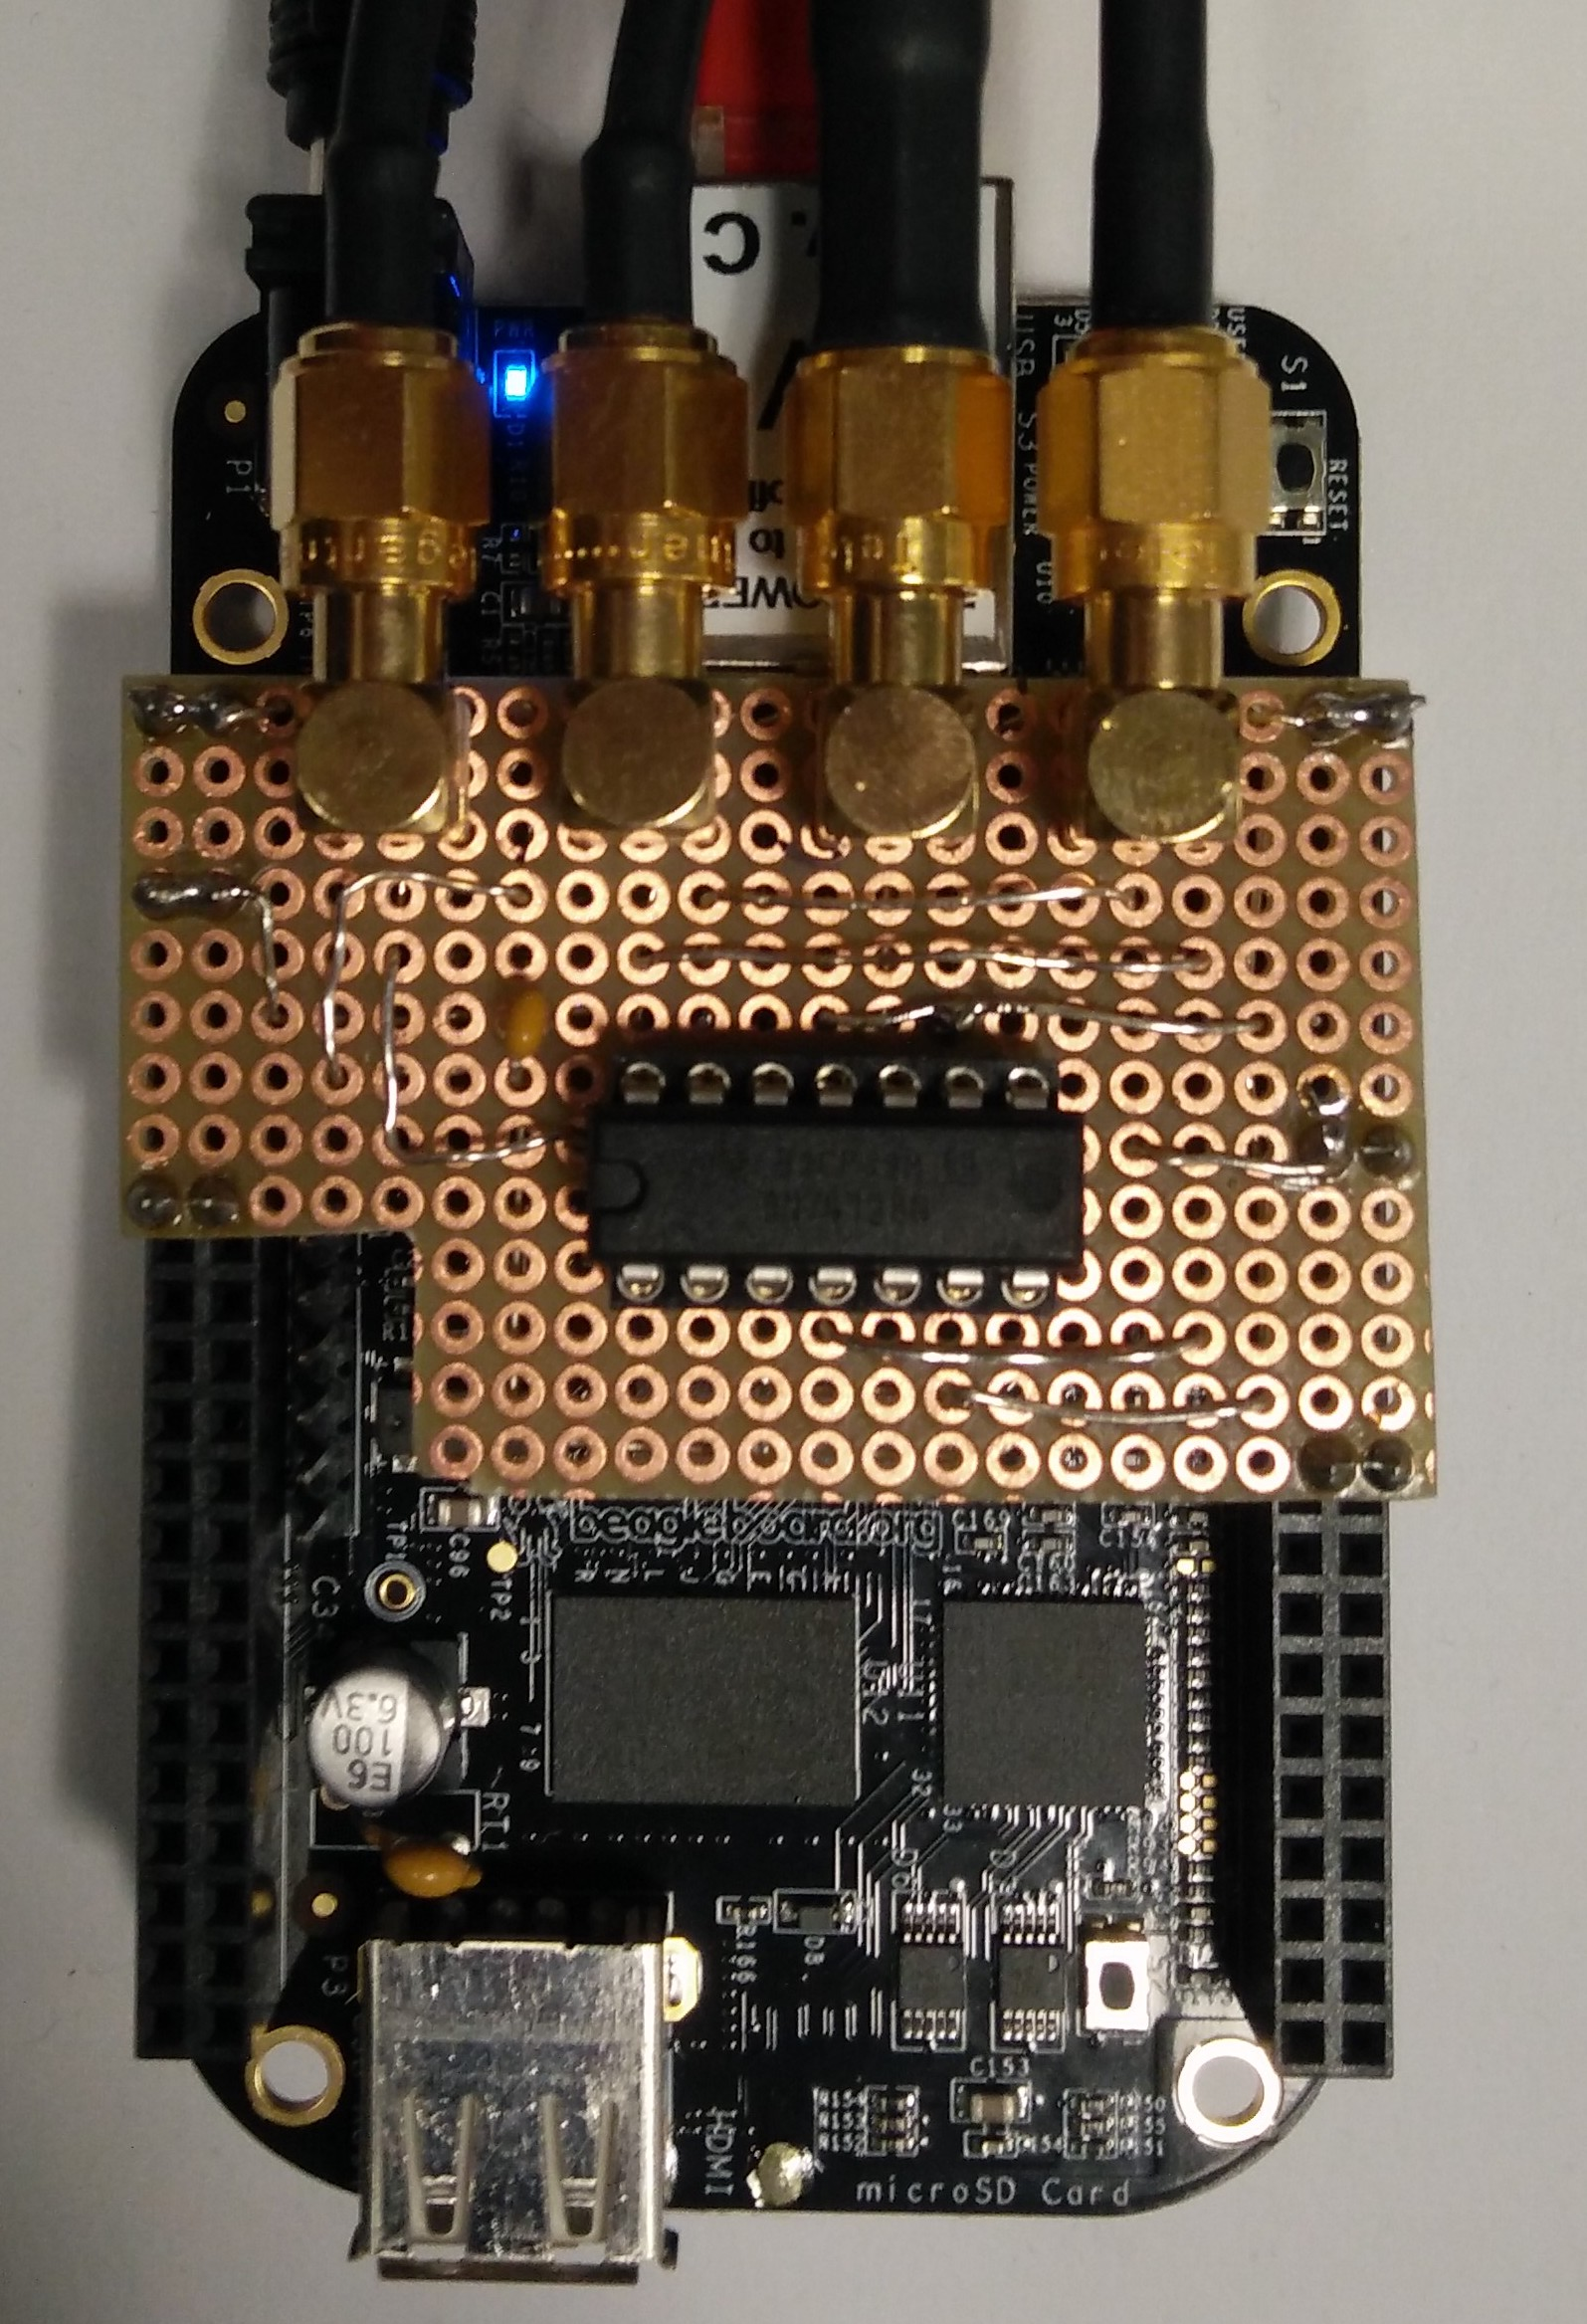
\includegraphics[width=.6\linewidth]{images/circuits/line-driver/board.jpg}
    \captionsetup{width=.8\linewidth}
    \caption{Picture of the trigger hub on the \gls{bbb}. The \gls{bbb} is
connected with the \gls{lan} via cable. The trigger hub forwards the signal
to the oscilloscope, the camera and the two \gls{dds}.}
  \end{minipage}
\end{figure}

\chapter{Acousto-Optics}

\section{Elastic Waves in Solids}
\section{Transducer}


\end{document}
